\newpage
\section{Proposal for classification of optimization approaches}
\label{ch:Proposal}

% TODO:
% - Deriving:
%     - SAS Taxonomy by Krupitzer et al
%     - How did Krupitzer get to his taxonomy?
%     - 5W+1H questions
%     - Classification proposed by: The Application of ML
% - Proposing:
%     - Explain each part:
%         - Purpose
%         - Time
%         - Technique
%         - Location
%         - Concern
%     - What to explain:
%         - Why?
%         - How is it different from the other properties?

% \begin{itemize}
%     \item Deriving a classification for optimization approaches for Self-Adaptive Systems.
%     \item Proposing a classification for optimization approaches for Self-Adaptive Systems.
% \end{itemize}

% \paragraph*{Literature for this section:} \begin{itemize}
%     \item "The Application of Machine Learning in Self-Adaptive Systems: A Systematic Literature Review" \cite{ApplicationOfMachineLearning}
% \end{itemize}

% TODO: Deriving a classification}
% TODO: reference for MAPE

% TODO: FUSION and other OA just update a knowledge base (MAPE-K) and dont directly adapt the system
% so maybe RAC is not the perfect name for that category: changing structure vs providing knowledge
% approach: not if RAC is internal/external but if the OA is internal/external
% This would also make the classification more relevant!
When thinking about how to classify optimization approaches for Self-Adaptive Systems,
one must realize that an optimization approach for Self-Adaptive Systems is really just
a Self-Adaptive System of a Self-Adaptive System.

Because of this the proposed classification for optimization approaches for Self-Adaptive Systems
should be based upon the same principles as the classification for Self-Adaptive Systems
and it should use the same terminology.

Following Krupitzer's et al, 2015\cite*{SurveyOnEngineeringApproaches} taxonomy for \acrlong{sas},
a classification for \acrlong{oa} of \acrshort{sas} should answer 
the 5W+1H questions by Salehie and Tahvildari, 2009\cite*{LandscapeAndResearchChallenges}.
These questions are:
\begin{itemize}
    \item Where is the need for change?
    \item When should a change occur?
    \item What should be changed?
    \item Why should something be changed?
    \item Who should change something?
    \item How should something be changed?
\end{itemize}

The process of optimizing \acrlong{sas} can be split into multiple parts 
using the MAPE-K (Monitor-Analyze-Plan-Execute with Knowledge) feedback loop by Kephart and Chess, 2003\cite*{VisionOfAutonomicComputing}.
Each part of the MAPE-K feedback loop can be mapped to the process of optimization in the following way:
\begin{itemize}
    \item Firstly the optimization approach has to constantly monitor the Self-Adaptive System and its context.
    \item The data gathered from monitoring can then be analyzed to decided wether or not an optimization is necessary and what should be optimized.
    \item After deciding that something should be optimized, there needs to be a plan on how to optimize.
    \item Lastly the planned optimization can be executed.
    \item For all of this the optimization approach requires knowledge about the Self-Adaptive System and its context.
\end{itemize}

% TODO: Proposing a classification

\begin{figure}
    \centering
    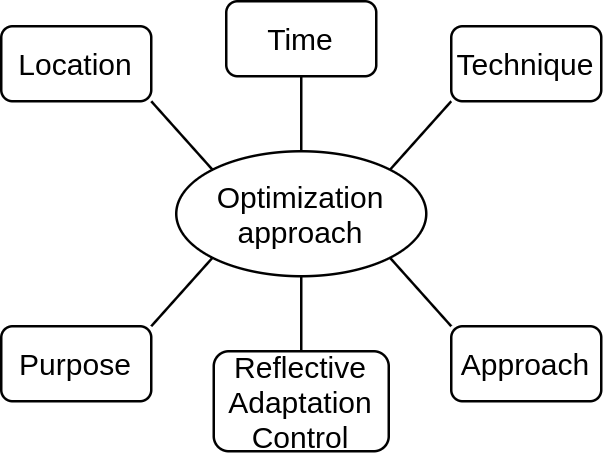
\includegraphics[width=0.6\columnwidth]{images/ClassificationProposal-Proposal.png}
    \caption{The proposed classification for Optimization Approaches for Self-Adaptive Systems}
\end{figure}

\subparagraph*{Location}
Where in the system is an optimization necessary? \\

\begin{itemize}
    \item Adaptation control
    \item Level
    \item Technique
    \item Time
\end{itemize}

\subparagraph*{Time}
When are optimizations performed? \\
Similarly to \acrshort{sas}, \acrlong{oa}[es] can be differentiated by comparing when they perfom optimizations.
There are three different phases during the lifetime of a Self-Adaptive System where optimizations can occur.
These are:
\begin{itemize}
    \item at the runtime of the system
    \item during the design time of the system
    \item while training the system
\end{itemize}
The training phase can happen in parallel to the run and design time of the system.
Examples for this would be when the inital parameters for a Self-Adaptive System are choosen by training a domain model
or when generating a new model for the system by training an updated domain model parallel to the running system.

\subparagraph*{Technique}
What gets changed to perform the optimization? \\
\begin{itemize}
    \item ---
\end{itemize}

\subparagraph*{Purpose}
Why should an optimization occur? \\
The most important question for any optimization is: What influences the need for an optimization.
Just like with Self-Adaptive Systems this can be caused by changes in context, the system itself or updated requirements for the system.
Additionally an optimization might be necessary if for example the system detects that its current adaptation control can be improved.

\begin{itemize}
    \item Changes in context, the system itself or requirements for the system.
    \item Detection of suboptimal adaptation logic.
\end{itemize}

% TODO: Approach outside of Adaptation Control because of the original meaning
% of the question: level of automation vs human interaction.
% Self-Adaptive Systems: trivially should only be adapted by themselves.
% Optimization approaches: there might be human intervention necessary -> ML: learning trap, unpredicatability
\subparagraph*{Approach}
Who is responsible for performing the optimization? \\
\begin{itemize}
    \item An internal component of the system
    \item An external actor
\end{itemize}

\subparagraph*{Reflective Adaptation Control}
How is the optimization applied to the system? \\
Just like the Self-Adaptive System can be described by its Adaptation Control,
which is responsible for applying changes to the system,
an optimization approach can also be described by how it applies its optimizations to the system.
In reference to FORMS by Weyns et al., 2012\cite*{FORMS}, which uses reflective operations to change
components in the system, the Adaptation Control of the optimization approach will be called Reflective Adaptation Control.

\begin{itemize}
    \item ---
\end{itemize}

\subparagraph*{MAPE Mapping}
\begin{tabular}{|c|c|}
    \hline
    MAPE & OA \\
    \hline
    Monitor & \\
    \hline
    Analyze & \\
    \hline
    Plan & Technique \\
    \hline
    Execute & Reflective Adaptation Control \\
    \hline
\end{tabular}

\subparagraph*{5W+1H Mapping}
\begin{tabular}{|c|c|}
    \hline
    5W+1H & OA \\
    \hline
    Where & Location\\
    \hline
    When & Time \\
    \hline
    What & Technique \\
    \hline
    Why & Purpose \\
    \hline
    Who & Approach \\ % TODO: part of the RAC?
    \hline
    How & Reflective Adaptation Control \\
    \hline
\end{tabular}